\chapter{Fonctionnement général}
\begin{figure}[H]
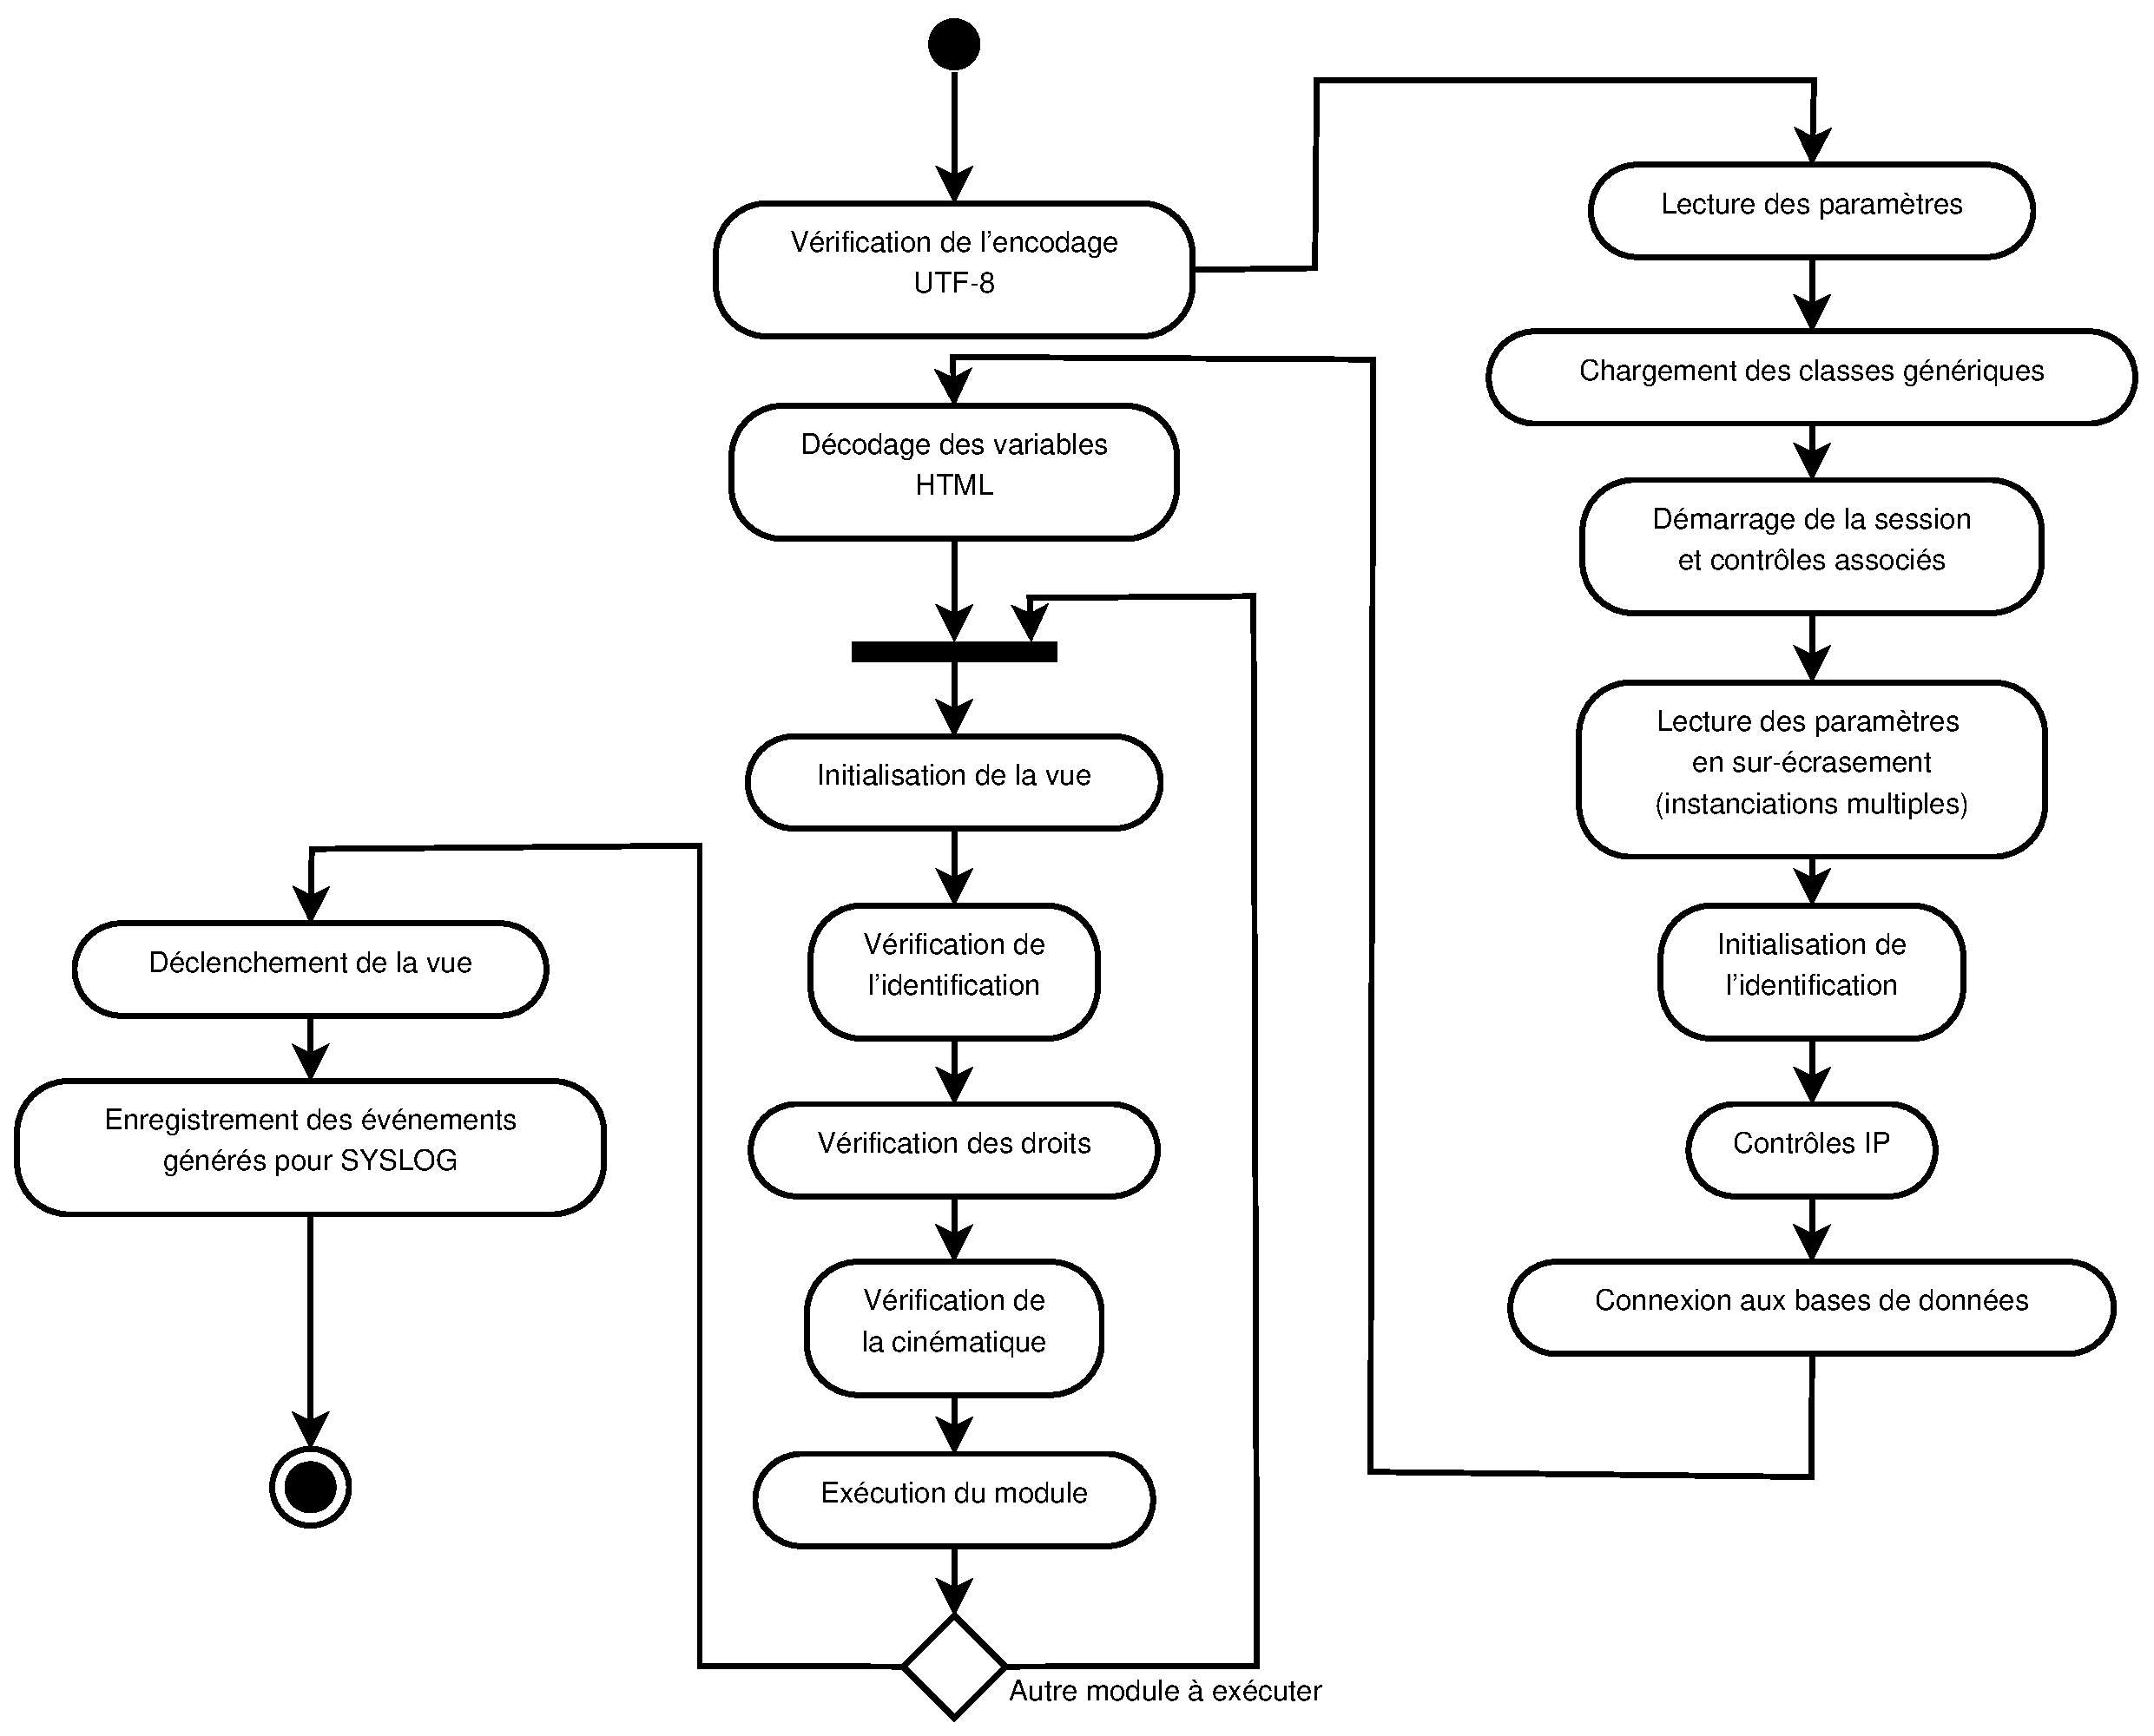
\includegraphics[width=1.2\linewidth]{dessin/synopsis}
\caption{Synopsis général de fonctionnement du contrôleur}
\end{figure}



\section{Synopsis}

L'appel de toute page dans l'application passe nécessairement par l'ensemble de ces étapes :
\begin{itemize}
\item vérification que l'encodage des caractères transmis respecte bien l'encodage utf-8
\item lecture des paramètres
\item chargement des classes génériques utilisées systématiquement
\item démarrage de la session, et ajout de contrôles (durée de la session ouverte...)
\item lecture des paramètres en sur-écrasement, ce qui permet des implémentations multiples avec le même code
\item initialisation de l'identification
\item contrôles de cohérence IP (vérification que, pour une même session, l'adresse IP ne change pas)
\item lancement des connexions aux bases de données (par défaut, deux connexions : une pour la base des droits, l'autre pour les données applicatives)
\item décodage des variables HTML encodées (protection contre les attaques de type XSS)
\item traitement du module demandé :
\begin{itemize}
\item initialisation, le cas échéant, de la vue associée 
\item vérification de l'identification, ou déclenchement des procédures d'identification
\item vérification des droits nécessaires pour accéder au module
\item vérification, le cas échéant, de la cinématique : les opérations de modification ne devraient être possibles que si l'opération précédente correspond à l'affichage du formulaire de saisie
\item exécution du module
\item analyse du code de retour du module, et enchaînement le cas échéant sur un autre module
\end{itemize}
\item déclenchement de la vue 
\item enregistrement, le cas échéant, des messages destinés à SYSLOG (messages systèmes)
\end{itemize}

\section{Organisation des dossiers}
Les fichiers sont organisés selon cette arborescence :
\begin{itemize}
\item \textbf{database} : dossier de travail contenant la description de la base de données, la documentation pour les développeurs, les scripts. Le dossier doit être supprimé lors de la mise en production
\item \textbf{display} : le seul dossier accessible. Il contient tous les fichiers nécessaires pour gérer l'affichage :
\begin{itemize}
\item \textbf{CSS} : les feuilles de style
\item \textbf{images} : les icônes et images utilisées dans l'affichage des pages
\item \textbf{javascript} : l'ensemble des librairies Javascript utilisées
\item \textbf{templates} : les modèles de documents utilisés par Smarty (cf. \ref{smarty}, \textit{\nameref{smarty}}, page \pageref{smarty})
\item \textbf{templates\_c} : dossier utilisé par Smarty pour compiler les templates. Ce dossier doit être accessible en écriture par le serveur Web
\end{itemize}
\item \textbf{doc} : ancien dossier, contenant un mécanisme de gestion de la documentation en ligne. N'est plus utilisé actuellement, mais pourrait être employé le cas échéant
\item \textbf{framework} : le code de base du framework. Il comprend :
\begin{itemize}
\item \textbf{droits} : dossier permettant de gérer les droits 
\item \textbf{identification} : gestion de la connexion des utilisateurs
\item \textbf{import/import.class.php} : classe créée il y a quelques années pour gérer les imports (obsolète en grande partie)
\item \textbf{ldap/ldap.class.php} : connexion à un annuaire LDAP et récupération d'informations
\item \textbf{navigation} : programmes utilisés pour générer le menu et décoder les actions demandées à partir du fichier XML les contenant
\item \textbf{translateId/translateId.class.php} : classe permettant de transcoder les identifiants des enregistrements de la base de données, pour éviter les attaques par forçage de clé
\item de nombreux fichiers utilisés par le framework, dont le contrôleur (controller.php), des fonctions génériques (fonctions.php)...
\item \textbf{vue.class.php} : les classes utilisées pour les vues (cf. \ref{vue} \textit{\nameref{vue}}, page \pageref{vue})
\end{itemize}
\item \textbf{install} : contient des scripts d'installation de la base de données (normalement à déplacer dans \textit{database}), et le fichier \textbf{readme.txt}, décrivant les dernières nouveautés
\item \textbf{locales} : dossier contenant les fichiers de langue (fr.php et en.php)
\item \textbf{modules} : dossier contenant le code spécifique de l'application. Il est organisé ainsi :
\begin{itemize}
\item \textbf{classes} : les classes nécessaires pour l'application
\item \textbf{example} : des exemples de codage
\item les autres dossiers sont libres et contiennent les modules de l'application
\item \textbf{beforeDisplay.php} : fichier appelé systématiquement avant l'affichage des pages HTML
\item \textbf{beforesession.inc.php} : fichier appelé systématiquement avant le démarrage de la session. Il permet de déclarer les librairies qui sont nécessaires pour instancier des classes stockées en variables de session
\item \textbf{common.inc.php} : fichier appelé systématiquement avant le traitement des modules
\item \textbf{fonctions.php} : fonctions déclarées par le programmeur et disponibles dans toute l'application 
\item \textbf{postLogin.php} : script exécuté uniquement quand un utilisateur s'est identifié
\end{itemize}
\item \textbf{param} : dossier contenant les paramètres de l'application :
\begin{itemize}
\item \textbf{actions.xml} : fichier contenant la description de l'ensemble des modules utilisables, avec les droits associés et le type de vue à utiliser
\item \textbf{menu.xml} : description du menu qui sera généré
\item \textbf{param.default.inc.php} : les paramètres par défaut
\item \textbf{param.inc.php} : paramètres en écrasement, spécifiques de l'implémentation. Ce fichier n'est jamais livré lors des mises à jour, pour éviter la suppression des paramètres de base de données, par exemple
\item \textbf{param.inc.php.dist} : fichier d'exemple de \textit{param.inc.php}, à renommer et à mettre à jour lors de l'installation d'une nouvelle implémentation
\end{itemize}
\item \textbf{plugins} : dossier contenant les bibliothèques tierces, comme Smarty, ObjetBDD (maintenant intégré au framework)...
\item \textbf{temp} : dossier de stockage temporaire, qui doit être accessible en écriture au serveur web. Les fichiers présents dans celui-ci ont une durée de vie de 24 heures (suppression lors de la connexion d'un utilisateur)
\item \textbf{test} : dossier utilisé pour réaliser certains tests. Doit être systématiquement supprimé lors de la mise en production
\end{itemize}

Seuls le fichier index.php, à la racine, les dossiers display et test sont accessibles directement. Les autres dossiers sont protégés par des fichiers .htaccess.

\section{Paramètres}\label{param}

Les paramètres utilisés dans l'application sont gérés avec 3 fichiers différents :
\begin{itemize}
\item \textbf{param/param.default.inc.php} : contient l'ensemble des paramètres utilisés ;
\item \textbf{param/param.inc.php} : contient ceux issus du fichier précédent, qui sont adaptés à l'implémentation ;
\item \textbf{param.ini} : fichier contenant les paramètres spécifiques du nom DNS de l'application (par exemple, schéma particulier associé au nom du site). Pour plus d'informations sur ce point, consultez le chapitre \ref{dnsmultiple} \textit{\nameref{dnsmultiple}}, page \pageref{dnsmultiple}.
\end{itemize}

Voici la description de l'ensemble des paramètres :

\subsection{Paramètres généraux}
% \usepackage{array} is required
\begin{longtable}{|p{5cm}|p{8cm}|}
\hline
\textbf{Variable} & \textbf{Signification} \\
\hline
\endhead
APPLI\_version & Numéro de version de l'application \\ 
\hline 
APPLI\_versiondate & Date de la version \\ 
\hline 
language & Langue par défaut \\
\hline
DEFAULT\_formatdate & Format par défaut d'affichage des dates\\
\hline
navigationxml & nom du fichier XML contenant la description des modules exécutables\\
\hline
APPLI\_session\_ttl & durée de la session, en secondes\\
\hline
APPLI\_cookie\_ttl & durée de vie par défaut des cookies, en secondes\\
\hline
APPLI\_path\_stockage\_session & obsolète\\
\hline
LOG\_duree & Durée de conservation des traces des actions réalisées, en jours\\
\hline
APPLI\_mail & Adresse pour déclarer les incidents (mail ou non)\\
\hline
APPLI\_titre & Nom de l'application qui sera affiché (cas où le code est utilisé par plusieurs entrées différentes) \\
\hline
APPLI\_code & Code interne de l'application. Utilisé dans certains cas\\
\hline
APPLI\_fds & Feuille de style utilisée par défaut (obsolète)\\
\hline
APPLI\_address & Adresse DNS de l'application. Utilisée en cas d'identification CAS (adresse de retour)\\
\hline
APPLI\_modeDeveloppement & si à true, certaines opérations sont réalisées dans un contexte de développement (affichage de messages, recalcul systématique du menu...)\\
\hline
APPLI\_notSSL & utilisé en développement, si l'application ne fonctionne pas en mode SSL (déconseillé) \\
\hline
APPLI\_utf8 & systématiquement à true (plus de support des autres encodages)\\
\hline
APPLI\_menufile & nom du fichier XML contenant la description du menu\\
\hline
APPLI\_temp & nom du dossier utilisé pour stocker les fichiers temporaires\\
\hline
APPLI\_moduleDroitKO & nom du module appelé en cas de refus d'accès pour un problème de droits \\
\hline
APPLI\_moduleErrorBefore & nom du module appelé en cas de problème lié à la cinématique de l'application\\
\hline
APPLI\_moduleNoLogin & nom du module appelé en cas d'échec d'identification \\
\hline
paramIniFile & nom du fichier contenant les paramètres spécifiques liés au DNS utilisé (\textit{cf.} \ref{dnsmultiple} \textit{\nameref{dnsmultiple}}, page \pageref{dnsmultiple}) \\
\hline
SMARTY\_param & Paramètres utilisés par le moteur de templates SMARTY\\
\hline
SMARTY\_variables & variables systématiquement transmises à SMARTY et utilisées lors de l'affichage général\\
\hline
ERROR\_display & Affiche les erreurs à l'écran (mode développement)\\
\hline
OBJETBDD\_debugmode & 0 : pas d'affichage de message d'erreur, 1, affichage des messages d'erreur, 2 : affichage de toutes les commandes SQL générées par ObjetBDD \\
\hline
ADODB\_debugmode & obsolète \\
\hline
\caption{Variables générales de l'application}
\end{longtable} 

\subsection{Identification}\label{paramident}
\begin{longtable}{|p{5cm}|p{8cm}|}
\hline
\textbf{Variable} & \textbf{Signification} \\
\hline
\endhead
ident\_type & Type d'identification supporté. L'application peut gérer \textbf{BDD} (uniquement en base de données),\textbf{LDAP} (uniquement à partir d'un annuaire LDAP) \textbf{LDAP-BDD} (d'abord identification en annuaire LDAP, puis en base de données), \textbf{CAS} (serveur d'identification \textit{Common Access Service}), et enfin \textbf{HEADER} (identification derrière un proxy qui fournit le login dans une variable d'entête HTTP)\\
\hline
CAS\_plugin & Nom du plugin utilisé pour une connexion CAS \\
\hline
CAS\_address & Adresse du serveur CAS\\
\hline
CAS\_port & Systématiquement 443 (connexion chiffrée)\\
\hline
LDAP & tableau contenant tous les paramètres nécessaires pour une identification LDAP \\
\hline
ident\_header\_login\_var & par défaut, AUTH\_USER. Nom de la variable qui contiendra le login dans le cas d'une identification en mode HEADER (le radical HTTP\_  ne doit pas être indiqué) \\
\hline
privateKey & clé privée utilisée pour générer les jetons d'identification \\
\hline
pubKey & clé publique utilisée pour générer les jetons d'identification \\
\hline
tokenIdentityValidity & durée de validité, en secondes, des jetons d'identification\\
\hline
\caption{Variables utilisées pour paramétrer l'identification}
\end{longtable}

Voici le contenu des variables du tableau LDAP : 
\begin{longtable}{|p{5cm}|p{8cm}|}
\hline
\textbf{Variable} & \textbf{Signification} \\
\hline
\endhead
address &  adresse de l'annuaire\\
\hline
port & 389 en mode non chiffré, 636 en mode chiffré\\
\hline
rdn & compte de connexion, si nécessaire \\
\hline
basedn & base de recherche des utilisateurs\\
\hline
user\_attrib & nom du champ contenant le login à tester\\
\hline
v3 & toujours à \textit{true}\\
\hline
tls & \textit{true} en mode chiffré\\
\hline
groupSupport & \textbf{true} si l'application recherche les groupes d'appartenance du login dans l'annuaire\\
\hline
groupAttrib & Nom de l'attribut contenant la liste des groupes d'appartenance\\
\hline
commonNameAttrib & Nom de l'attribut contenant le nom de l'utilisateur\\
\hline
mailAttrib & Nom de l'attribut contenant l'adresse mail de l'utilisateur\\
\hline
attributgroupname & Attribut contenant le nom du groupe lors de la recherche des groupes (cn par défaut)\\
\hline
attributloginname & attribut contenant les membres d'un groupe\\
\hline
basedngroup & base de recherche des groupes \\
\hline
\caption{Variables utilisées pour paramétrer l'accès à l'annuaire LDAP}
\end{longtable}

\subsection{Connexions aux bases de données}

Deux connexions sont systématiquement implémentées : l'une à la base de données contenant la gestion des droits, et l'autre à celle contenant les données propres à l'application.
\begin{longtable}{|p{5cm}|p{8cm}|}
\hline
\textbf{Variable} & \textbf{Signification} \\
\hline
\endhead
BDD\_login & compte de connexion à la base de données \\
\hline
BDD\_passwd & mot de passe associé\\
\hline
BDD\_dsn & adresse de la base de données sous forme normalisée\\
\hline
BDD\_schema & schéma utilisé (plusieurs schémas peuvent être décrits, en les séparant par une virgule - fonctionnement propre à Postgresql)\\
\hline
GACL\_dblogin & compte de connexion à la base de données des droits\\
\hline
GACL\_dbpasswd & mot de passe associé\\
\hline
GACL\_dsn & adresse normalisée \\
\hline
GACL\_schema & schéma utilisé\\
\hline
GACL\_aco & nom du code de l'application utilisé dans la gestion des droits (\textit{cf.} \ref{droits} \textit{\nameref{droits}}, page \pageref{droits} )\\
\hline


\caption{Variables utilisées pour paramétrer les connexions}
\end{longtable}

Il est possible de créer des comptes séparés, voire de ne donner accès qu'en lecture à la base des droits (à l'exception de la table \textit{log}, qui contient la trace de toutes les actions demandées).

\section{Gestion des messages}

Une classe est instanciée systématiquement pour gérer les messages, la classe \textit{Message}. Deux types de messages sont pris en compte :
\begin{itemize}
\item les messages envoyés au navigateur, à destination de l'utilisateur ;
\item les messages enregistrés dans Syslog, le mécanisme de gestion des messages systèmes de Linux.
\end{itemize}

Les messages sont enregistrés dans un tableau, qui sera ensuite dépilé pour générer les textes soit à afficher, soit à stocker dans Syslog.

La classe dispose des fonctions suivantes :
\begin{longtable}{|p{5cm}|p{8cm}|}
\hline
\textbf{fonction} & \textbf{Objectif} \\
\hline
\endhead
\_\_construct(\$displaySyslog = false) & Constructeur de la classe. La variable permet d'indiquer si les messages destinés à Syslog sont également affichés à l'écran (mode par défaut en développement) \\
\hline
set(\$value) & Ajoute un nouveau libellé utilisateur \\
\hline
setSyslog(\$value) & Ajout un nouveau message système \\
\hline
get() & Retourne le tableau contenant l'ensemble des messages, avec ou sans les messages systèmes, selon le mode indiqué dans le constructeur \\
\hline
getAsHtml() & Formate les messages pour les envoyer au navigateur. Chaque message est séparé par un retour à la ligne. Les libellés sont encodés en HTML avant d'être envoyés \\
\hline
sendSyslog() & Génère un message dans Syslog. Actuellement, le message est toujours de type NOTICE. \\
\hline

\caption{Fonctions utilisables dans la classe Message}
\end{longtable}

Les messages sont systématiquement transmis à la vue Smarty, et l'envoi des messages systèmes est la dernière action réalisée avant l'affichage de la vue.

\chapter{Décrire les actions}\label{labelxml}

Les actions possibles dans le logiciel sont décrites dans un fichier, par défaut \textit{param/actions.xml}. C'est un fichier XML dont la racine s'appelle \textit{navigation}. 

Une action est la conjonction entre un contexte et une opération, par exemple \textit{poissonList} pour afficher la liste des poissons, \textit{poissonChange} pour afficher la page de modification d'un poisson, \textit{poissonWrite} ou \textit{poissonDelete} pour déclencher l'écriture en base de données.

Dans le contexte de ce framework, l'action s'appelle \textit{module} (nom du champ transmis depuis le navigateur). L'attribut \textit{action} contient le nom du fichier PHP appelé. Il est associé à l'attribut \textit{param}, qui permet d'indiquer le détail de l'action à réaliser (par exemple, \textit{list} ou \textit{change}).

Voici la liste des attributs disponibles pour un module (ou une action) :
\begin{longtable}{|p{2.5cm}|c|p{9cm}|}
\hline
\textbf{Attribut} & \textbf{Requis} & \textbf{Signification} \\
\hline
\endhead
action & X & nom de la page PHP à exécuter (accès relatif depuis la racine de l'application) \\
 \hline
param &  & paramètre analysé dans la page, pour savoir quelle action doit être réalisée. Par convention, les actions possibles sont les suivantes : list, read, change, write, delete, ou autre action \\
 \hline
droits &  & Liste des droits nécessaires pour exécuter l'action. Si plusieurs droits sont possibles, ils doivent être séparés par une virgule\\
 \hline
loginrequis & & Indique, en l'absence de droits spécifiques, si l'action nécessite d'être connecté. Vaut 1 si la connexion est requise\\
 \hline
modulebefore & & Pour les opérations d'écriture, permet d'indiquer le nom du module qui doit impérativement être exécuté avant. Cela limite les risques d'attaques de type CSRF et les rafraîchissements intempestifs dans les formulaires. Plusieurs modules peuvent être indiqués, en les séparant par une virgule\\
 \hline
retourok & & indique le nom du module qui sera exécuté si le code de retour (variable \$module\_coderetour) vaut 1 \\
 \hline
retourko & & indique le nom du module qui sera exécuté si le code de retour (variable \$module\_coderetour) vaut -1 (échec d'exécution) \\
 \hline
type & (X) & pour les modules envoyant des données au navigateur, indique le type de la vue qui sera utilisée. Les valeurs possibles sont smarty ou html (même vue), ajax, pdf, csv  \\
 \hline
droitko & & nom du module appelé si les droits ne sont pas suffisants pour exécuter l'action demandée \\
\hline 
 
 \caption{Liste des attributs utilisables pour décrire une action}\label{actions}
\end{longtable}

Le module \textit{model} n'est pas analysé, il sert à montrer l'ensemble des options possibles. 

Le module \textit{default} correspond au module appelé par défaut, si l'application est appelée sans indiquer de nom de module (variable \textit{module} non transmise soit dans le lien, soit dans le formulaire).

Voici quelques exemples d'utilisation :
\begin{lstlisting}
	<appliList action="framework/droits/appli.php" param="list" droits="admin" retourlogin="1"  type="smarty" />
	<appliDisplay action="framework/droits/appli.php" param="display" droits="admin"  type="smarty"/>
	<appliChange action="framework/droits/appli.php" param="change" droits="admin"  type="smarty"/>
	<appliWrite action="framework/droits/appli.php" param="write" droits="admin" retourok="appliDisplay" retourko="appliChange" modulebefore="appliChange" />
	<appliDelete action="framework/droits/appli.php" param="delete" droits="admin" retourok="appliList" retourko="appliChange"  modulebefore="appliChange"/>
\end{lstlisting}

Il s'agit des modules utilisés dans la gestion des droits. Ils nécessitent tous que l'utilisateur dispose du droit \textit{admin}. Une seule page est appelée (\textit{appli.php}), l'action à réaliser étant analysée à partir de l'attribut \textit{param}.

Les modules \textit{appliWrite} et \textit{appliDelete} ne génèrent pas directement d'affichage : ils sont là uniquement pour écrire des informations dans la base de données. Par contre, ils enchaînent, en fonction de leur code de retour, soit sur le réaffichage du formulaire de saisie, soit sur le retour au détail ou à la liste.
Ces deux modules ne peuvent être exécutés que si le précédent est \textit{appliChange}, c'est à dire si le formulaire de saisie a été affiché.

\chapter{Identifier les utilisateurs et gérer les droits}\label{droits}
\section{Identifier les utilisateurs}

Cinq modes d'identification sont prévus dans le logiciel :
\begin{itemize}
\item uniquement dans le logiciel (comptes stockés dans la base de données) ;
\item à partir d'un annuaire LDAP ;
\item d'abord en recherchant dans l'annuaire LDAP, puis ensuite dans la base des comptes de l'application (mode mixte) ;
\item auprès d'un serveur CAS ;
\item derrière un serveur d'identification, type LemonLdap\footnote{LemonLdap (\url{http://lemonldap-ng.org}) est un serveur proxy qui s'interface entre l'utilisateur et le serveur web de l'application. Il gère l'identification des utilisateurs, et n'autorise l'accès au serveur web applicatif que si elle est réussie}, qui fournit l'identification dans une variable HEADER.
\end{itemize}

L'identification retenue est déclarée dans les paramètres généraux (\textit{cf.} \ref{paramident} \textit{\nameref{paramident}}, page \pageref{paramident}).

Si l'identification à partir d'un annuaire LDAP ou d'un serveur CAS ne nécessite guère d'autres informations que celles décrites dans les paramètres, l'identification par base de données comprend des mécanismes particuliers pour protéger les mots de passe et limiter les risques associés. Voici les règles imposées lors de la création d'un mot de passe : 
\begin{itemize}
\item il doit avoir une longueur minimale de 8 caractères ;
\item il doit comporter 3 jeux de caractères différents (minuscules, majuscules, chiffres et autres caractères) ;
\item il n'est pas possible de réutiliser un mot de passe pour le même compte.
\end{itemize}

Les mots de passe sont salés (utilisation du login) et chiffrés (chiffrement SHA-256).

L'écran de création propose un bouton de génération automatique d'un mot de passe, qui devra être transmis à l'utilisateur, en lui demandant d'en changer (il peut modifier son mot de passe une fois connecté).

Dans sa version actuelle, le framework ne dispose pas d'un mécanisme de récupération par envoi de mails.

Les mots de passe n'expirent pas.

\subsection{Identification par HEADER}

Dans ce mode d'identification, le serveur web est placé derrière un serveur d'identification, appelé proxy d'identification. L'adresse de l'application pointe vers ce dernier. 

Le proxy gère la connexion de l'utilisateur, et fournit à l'application le login dans une variable configurable. Cette variable est accessible dans le tableau \$\_SERVER, par exemple \$\_SERVER["HTTP\_AUTH\_USER"].

Pour activer ce mécanisme, il faut modifier les paramètres suivants dans le fichier \textit{param.ini.php} (\textit{cf.} \ref{paramident} \textit{\nameref{paramident}}, page \pageref{paramident}) :
\begin{lstlisting}
$ident_type = "HEADER";
$ident_header_login_var = "AUTH_USER";
\end{lstlisting}

la variable ne doit pas contenir la racine HTTP\_ (une fonction l'extrait automatiquement).

\subsection{Ré-identification par jeton}

Par défaut, les sessions ont une durée de vie d'une heure. Dans certains cas de figure, il est souhaitable que l'utilisateur n'ait pas à ressaisir ses identifiants systématiquement.

Le framework peut générer un jeton chiffré après la première identification, qui sera analysé pour savoir si l'utilisateur peut être ré-identifié automatiquement.

Pour que ce mécanisme fonctionne, il faut :
\begin{itemize}
\item que le paramètre \textit{tokenIdentityValidity} ait une durée de validité supérieure à la durée de vie de la session. Il est raisonnable de ne pas fixer une durée de vie supérieure à une journée de travail (10 heures). Le cookie transmis est protégé ;
\item que les clés privée et publique, utilisées pour le chiffrement du jeton, soient accessibles au serveur web (variables \textit{privateKey} et \textit{publicKey}).
\end{itemize}

Le jeton est chiffré avec la clé privée, ce qui lui permet d'être lu, le cas échéant, par l'application. Il contient le login et la date d'expiration. 

Si l'utilisateur déclenche une déconnexion, le jeton est supprimé.

\section{Gérer les droits}

Les droits sont gérés selon le principe initialement utilisé dans la bibliothèque PHPGACL, aujourd'hui obsolète. 

Les logins sont déclarés dans des groupes organisés de manière hiérarchique : un groupe hérite des droits attribués à ses parents.

Les droits utilisés dans le logiciel sont associés à des groupes. Il est possible d'attribuer plusieurs droits à un même groupe, et un droit peut être détenu par des groupes différents.

Si le paramètre \textit{\$LDAP["groupSupport"]} est positionné à \textit{true}, les groupes dont fait partie le compte LDAP sont également récupérés, et peuvent être détenteurs de droits dans le logiciel (le nom des groupes est sensible à la casse).

Voici le schéma des tables utilisées pour gérer les droits :

\begin{figure}[H]
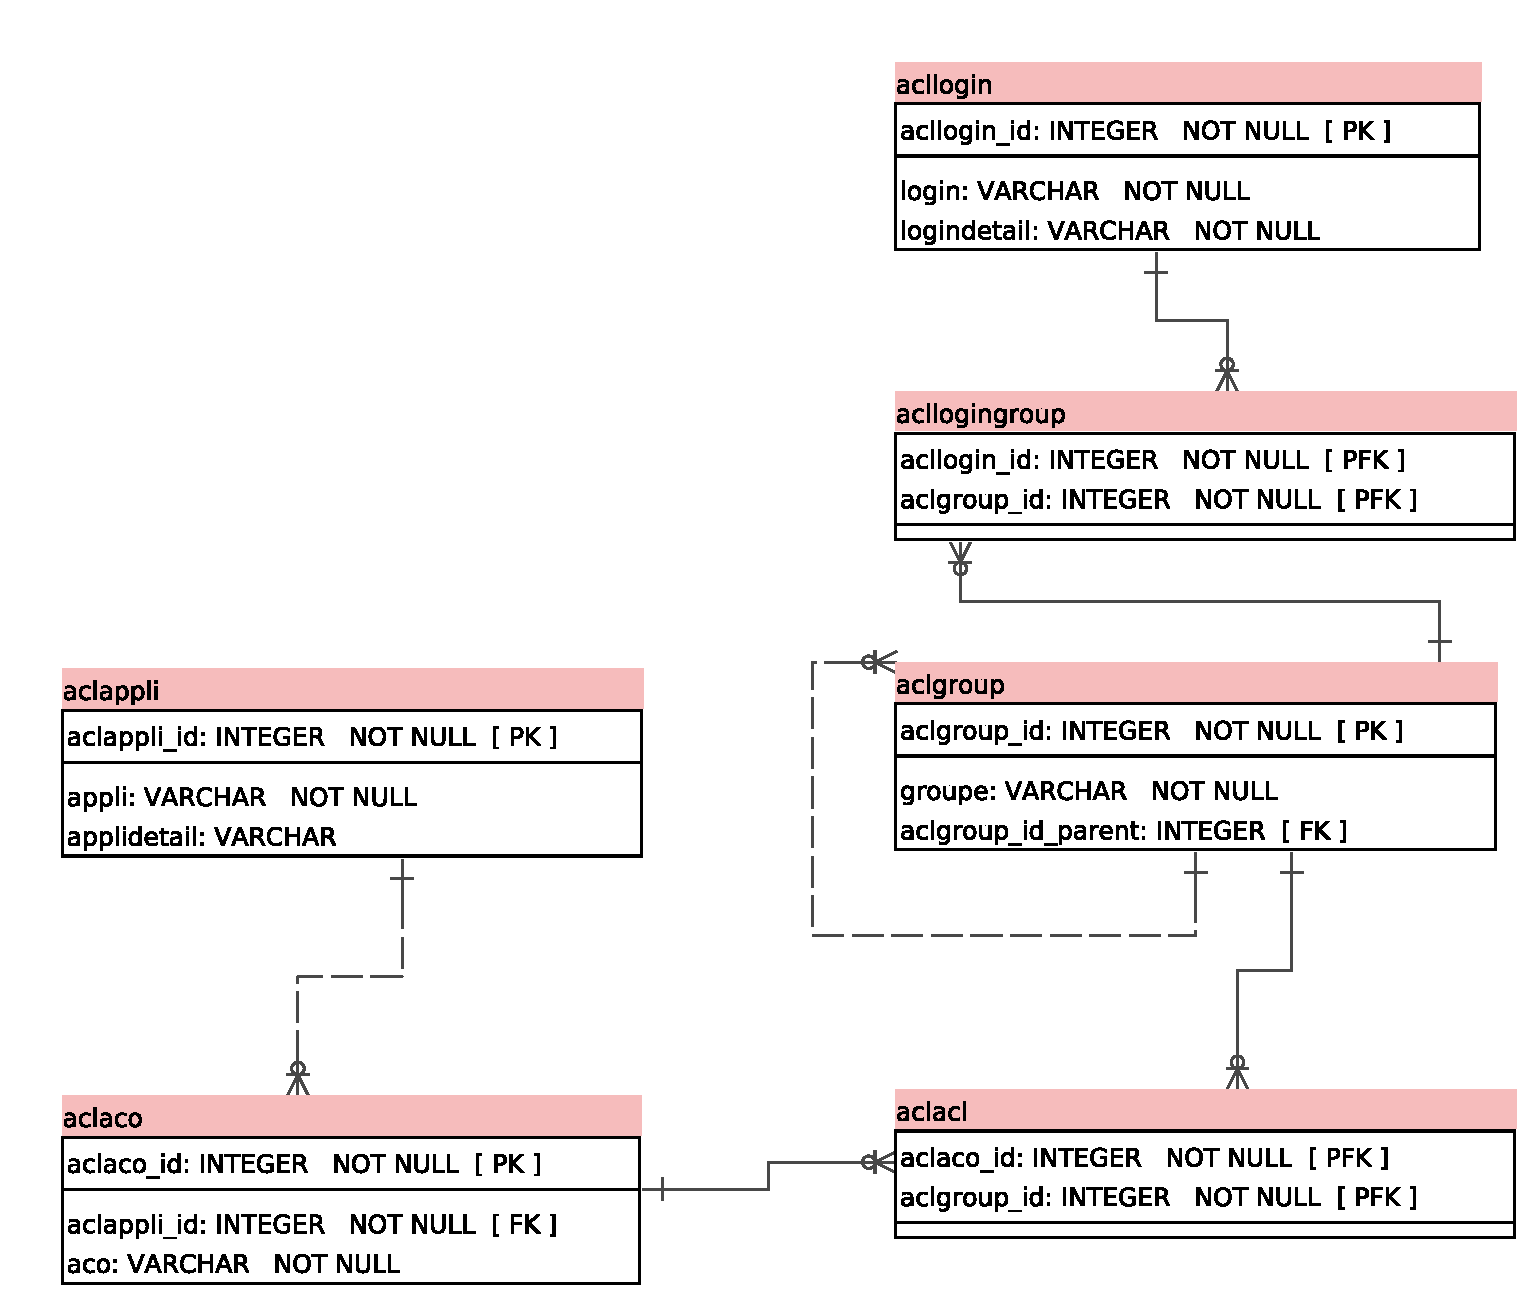
\includegraphics[width=\linewidth]{dessin/acl_only}
\caption{Schéma des tables utilisées pour gérer les droits}
\end{figure}

Voici la description des tables :
\begin{description}
\item[acllogin] Liste des logins utilisés. Si un compte est créé dans la base locale d'identification, un enregistrement est également créé dans cette table. Pour les identifications LDAP ou CAS, ils doivent être identiques. Si seuls les groupes LDAP sont utilisés pour un compte, il n'a pas besoin d'être décrit ici
\item[aclappli] Liste des applications gérées. Il est ainsi possible de gérer, à partir de la même base de données, plusieurs ensembles de droits, qui utilisent les mêmes logins
\item[aclaco] liste des droits déclarés dans l'application
\item[aclgroup] Liste des groupes contenant les logins, et qui détiennent les droits. Un groupe peut hériter d'un autre groupe. Les droits associés au groupe parent sont également attribués au groupe hérité.
\item[acllogingroup] table permettant de déclarer les logins associés à un groupe
\item[aclacl] table décrivant les droits détenus par un groupe
\end{description}

Le module d'administration permet de saisir toutes ces informations. Il faut que l'utilisateur dispose du droit \textit{admin}, c'est à dire faire partie du groupe \textit{admin} (configuration par défaut à l'initialisation de la base des droits) pour pouvoir accéder à ces fonctions.

\subsection{Créer un nouvel utilisateur}

Les utilisateurs peuvent être issus soit de l'annuaire LDAP, soit de la base interne. 
Pour créer un nouvel utilisateur dans la base locale :
\begin{itemize}
\item \textit{Administration $\rightarrow$ Liste des comptes }
\item \textit{Nouveau login}
\item renseignez au minimum le login.
\end{itemize}

\begin{figure}[H]
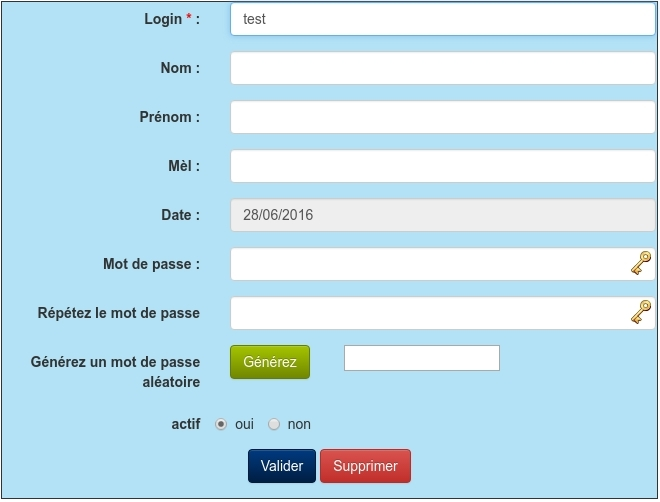
\includegraphics[width=\linewidth]{dessin/user_create}
\caption{Écran de saisie d'un login de connexion}
\end{figure}

Pour créer le mot de passe, vous pouvez cliquer sur le bouton \textit{Générez}, qui  en créera un automatiquement. Envoyez-le par mél à son destinataire (par \textit{copier-coller}), en lui demandant de le modifier à la première connexion (icône en forme de clé, dans le bandeau, en haut à droite).

Les mots de passe doivent respecter les règles suivantes :
\begin{itemize}
\item ils doivent avoir une longueur minimale de 8 caractères ;
\item ils doivent comprendre trois types de caractères différents parmi les minuscules, majuscules, chiffres et caractères de ponctuation ;
\item ils ne peuvent pas être réutilisés pour le même login ;
\item les mots de passe n'expirent pas.
\end{itemize}

Les mots de passe sont stockés sous forme d'empreinte, calculée en rajoutant un sel\footnote{chaîne de caractère rajoutée au mot de passe -- en général le login ou un identifiant -- qui permet d'éviter que deux mots de passe identiques, associés à deux logins différents, aient la même empreinte} et encodés en SHA256 : ils ne peuvent pas être retrouvés en cas de perte.

L'application n'intègre pas de module permettant de régénérer automatiquement un mot de passe en cas de perte : c'est au responsable applicatif d'en fournir alors un nouveau.

La création d'un compte entraîne la création d'une entrée identique dans la table des \textit{acllogin}, utilisée pour attribuer les droits.

Pour désactiver temporairement un compte, sélectionnez \textit{non} dans la zone \textit{actif}. Si le compte ne doit plus être utilisé, supprimez-le.

Attention : si le compte disposait des droits d'administration, assurez-vous que vous avez toujours un compte disposant des mêmes droits avant la suppression.

\subsection{Créer un login utilisé dans la gestion des droits}

Indépendamment du compte de connexion, qui peut être soit issu de la base interne, soit récupéré auprès d'un annuaire LDAP ou d'un serveur CAS, l'application a besoin de connaître les utilisateurs pour pouvoir leur attribuer des droits.

À partir du menu, choisissez \textit{Administration $\rightarrow$ ACL - logins}.

Vous pouvez modifier un login existant ou en créer un nouveau. Dans ce cas, vous devrez indiquer au minimum le login utilisé (identique à celui qui est employé pour la connexion à l'application : base de données interne, annuaire LDAP, serveur CAS).

\begin{figure}[H]
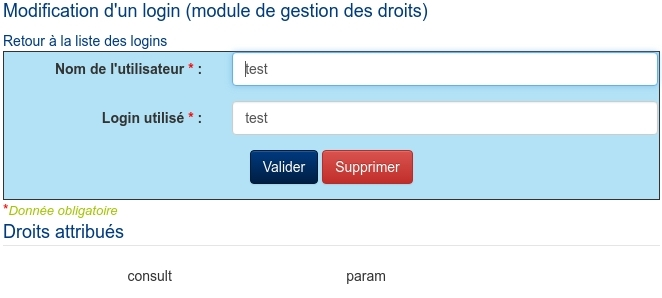
\includegraphics[width=\linewidth]{dessin/acl_login}
\caption{Écran de modification d'un login dans le module de gestion des droits}
\end{figure}


Sous l'écran de saisie figurent la liste des droits attribués à un login (en modification, le calcul n'est réalisé qu'à l'affichage de la page).

\subsection{Définir les groupes d'utilisateur}

Les groupes d'utilisateurs sont gérés selon un mécanisme d'héritage. Un groupe de haut niveau hérite des groupes précédents : si des droits ont été attribués à un groupe de niveau inférieur, un login associé à un groupe de niveau supérieur les récupère également.

Pour définir les groupes, dans le menu, choisissez \textit{Administration $\rightarrow$ ACL - groupes de logins}.

\begin{figure}[H]
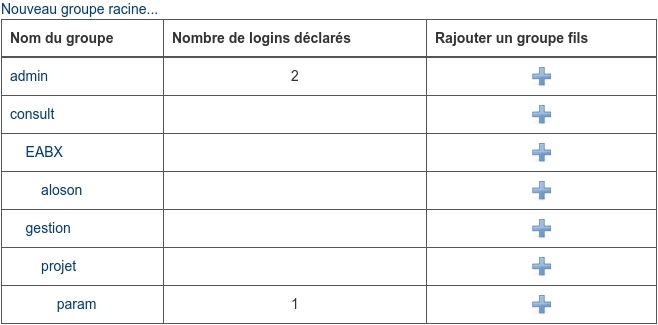
\includegraphics[width=\linewidth]{dessin/acl_groupe}
\caption{Liste des groupes de logins}
\end{figure}

Ainsi, le login déclaré dans le groupe \textit{param} récupérera les droits attribués aux groupes \textit{projet}, \textit{gestion} et \textit{consult}.

Pour créer un groupe, deux possibilités :
\begin{itemize}
\item soit le groupe est à la base d'une nouvelle branche : utilisez alors \textit{Nouveau groupe racine...} ;
\item soit le groupe hérite d'un autre groupe : cliquez sur le signe + (\textit{Rajouter un groupe fils}).
\end{itemize}

Vous pouvez indiquer les logins qui sont rattachés à ce groupe.


\subsection{Créer une application}
Le framework permet de gérer des droits différents pour des jeux de données différents, à partir du même code applicatif. Chaque couple \textit{logiciel} $\leftrightarrow$ \textit{base de données} constitue donc une \textit{application}, au sens de la gestion des droits.

Il est ainsi possible, à partir de la même base de données, de définir des droits différents selon les jeux de données utilisés (un jeu de données correspond à un schéma de base de données comprenant l'intégralité des tables applicatives).

À partir du menu, choisissez \textit{Administration $\rightarrow$ ACL - droits} :
\begin{figure}[H]
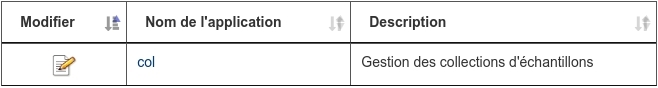
\includegraphics[width=\linewidth]{dessin/liste_appli}
\caption{Liste des applications déclarées}
\end{figure}

Pour créer une nouvelle application, choisissez \textit{Nouvelle application...}. 

\begin{figure}[H]
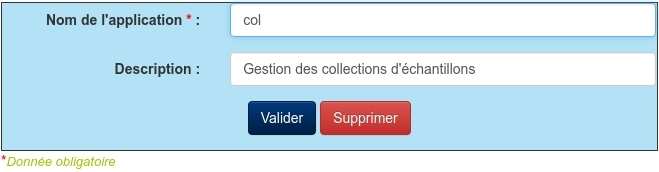
\includegraphics[width=\linewidth]{dessin/appli_change}
\caption{Écran de saisie d'une application}
\end{figure}

Le nom de l'application doit impérativement correspondre à la valeur \textit{\$GACL\_appli} dans les fichiers de paramètres : c'est ce qui permet au framework de savoir quels droits appliquer.

\subsection{Définir les droits utilisables dans l'application}

À partir de la liste des applications, cliquez sur le nom de celle pour laquelle vous voulez définir les droits utilisables. 
À partir de la liste, sélectionnez \textit{Nouveau droit...}.

\begin{figure}[H]
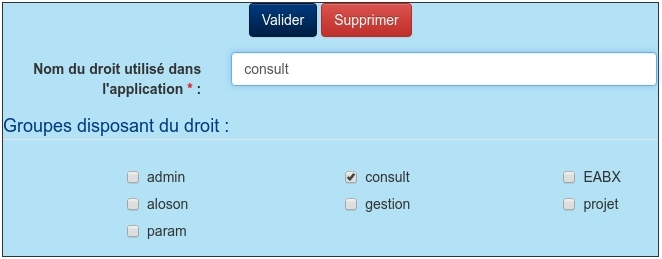
\includegraphics[width=\linewidth]{dessin/appli_droit}
\caption{Écran de saisie des droits associés à une application}
\end{figure}

Le nom du droit doit être celui défini dans le corps de l'application (les droits sont positionnés dans les fichiers \textit{param/actions.xml}, qui contient la liste des modules utilisables, et \textit{param/menu.xml}, qui sert à générer le menu).

Indiquez les groupes d'utilisateurs qui seront associés au droit courant.

\subsection{Cas particulier des groupes et des logins issus d'un annuaire LDAP}

Si vous avez paramétré l'application pour qu'elle s'appuie sur un annuaire LDAP pour gérer l'affectation des utilisateurs dans les groupes, vous n'êtes pas obligés de les déclarer explicitement dans le module de gestion des droits.

\subsubsection{Droits attribués à un groupe LDAP}

Tous les utilisateurs d'un groupe héritent d'un droit dans l'application.

\begin{itemize}
\item définissez le nom du groupe (en respectant la casse) dans le tableau des groupes d'utilisateurs ;
\item sélectionnez le nom de ce groupe dans les droits utilisables ;
\item tous les utilisateurs de l'annuaire LDAP récupéreront automatiquement les droits attribués à ce groupe.
\end{itemize}

\subsubsection{Droits attribués à un utilisateur particulier de l'annuaire LDAP}

Un utilisateur s'identifie auprès de l'annuaire LDAP, mais dispose de droits particuliers.

\begin{itemize}
\item créez son login dans la gestion des droits ;
\item rajoutez-le dans le groupe d'utilisateurs adéquat.
\end{itemize}